\documentclass[runningheads]{llncs}
%
\usepackage{graphicx}
\newcommand{\code}[1]{\texttt{#1}}

\def\bitcoin{
    \leavevmode
    \vtop{\offinterlineskip %\bfseries
    \setbox0=\hbox{B}
    \setbox2=\hbox to\wd0{\hfil\hskip-.03em
    \vrule height .3ex width .15ex\hskip .08em
    \vrule height .3ex width .15ex\hfil}
    \vbox{\copy2\box0}\box2}
}

\begin{document}
%
\title{Integrated Power Plant and Bitcoin Mining Economics}
%
\titlerunning{Bitcoin Mining Economics}
%
\author{Cal Abel\inst{1}\orcidID{0000-0003-2557-6746}}
%
\authorrunning{C. Abel}
%
\institute{Skylane Engineering, LLC, Atlanta GA 30306, USA 
\email{crabel@skylaneengineering.com}\\
\url{https://skylaneengineering.com}}
%
\maketitle
%
\begin{abstract}
Bitcoin mining can be a difficult process to understand much less model.
It is confounded by currency exchange rates and jurisdictional taxes along with rapid historical technological development.
This paper derives a framework for simplifying the modeling process.
It does so by first modeling trends in bitcoin miner performance showing that further gains in efficiency have plateaued.
It then derives the marginal utility of bitcoin treating the process of the block reward in a quantum mechanical framework.
Using the derived marginal utility, we present a universal cost basis and derive the economic model that formally takes into account uncertainty.
%
\keywords{bitcoin mining \and quantum mechanics \and statistical economics \and EROI \and Moore's Law.}
\end{abstract}



%%%%%%%%%%%%%%%%%%%%%%%%%%%%%%%%%%%%%%%%%%%%%%%%%%%%%%%%%%%%%%%%%%%%%%%%%%%%%%%%%%%%%%%%%%%%%%%%%%%
% Introduction
%%%%%%%%%%%%%%%%%%%%%%%%%%%%%%%%%%%%%%%%%%%%%%%%%%%%%%%%%%%%%%%%%%%%%%%%%%%%%%%%%%%%%%%%%%%%%%%%%%%
\section{Introduction}

Bitcoin mining has been something that has historically been relatively difficult to understand or to quantify the returns.
The primary objective of this paper is to arrive at a methodology that is firmly rooted in first principles and is simple and intuitive in application.

One of the chief problems that bitcoin has had is in managing the exchange rates and price fluctuations.
This has existed because the primary unit of account has not been fundamental and was tied to directly fiat currency.
The primary objective of this paper is to establish a universal and absolute measure of bitcoin's utility.

This is far easier said than done.
We need to understand how processing technology has evolved over time.
We will also discuss how to look at bitcoin mining in a more wholistic manner.
We also need to understand how bitcoin mining works at its deepest and most fundamental level.
Once we have these two components, we can derive the marginal utility of bitcoin.

From here we will develop the economic model.
We need to understand first how bitcoin mining can be integrated into the electric grid, as this understanding is what informs how we construct and think about the overall economic model.
It provides the overall constraints with in which we have to work.
This model will establish a cost basis using the universal metric of utility and simplify how we can account for the long term performance of the miners.

The concluding model will formally take into account the known uncertainty of the model, providing an uncertainty adjusted metric for project evaluation.
What is interesting is that this model shares a number of similarities with the concept of Energy Return on Investment, EROI.
EROI is a dimensionless measure of the amount of energy that one gets out of a power plant divided by the amount of energy input into the power plant.
One of the major shortfalls of EROI is that it does not take into account the uncertainty in the output of the generation source, which will be resolved by the approach taken here.

%%%%%%%%%%%%%%%%%%%%%%%%%%%%%%%%%%%%%%%%%%%%%%%%%%%%%%%%%%%%%%%%%%%%%%%%%%%%%%%%%%%%%%%%%%%%%%%%%%%
% Trends in Mining Performance
%%%%%%%%%%%%%%%%%%%%%%%%%%%%%%%%%%%%%%%%%%%%%%%%%%%%%%%%%%%%%%%%%%%%%%%%%%%%%%%%%%%%%%%%%%%%%%%%%%%
\section{Trends in Mining Performance}
Moore's Law is commonly thought of as being an axiom of computational power increases.
There are some very real physical limits to this trend that effect how well our silicone based chips perform.
To understand the trends in mining performance we need to first understand what these physical limitations are.
Once we have this understanding, we will look at trends in microprocessor performance over the last 48-years along with trends in computer hashing performance.
While transistor density is an important metric, it is not germane to the economics of bitcoin mining.
The single most important parameter is the energy utilization of the chip per operation conducted.

%%%%%%%%%%%%%%%%%%%%%%%%%%%%%%%%%%%%%%%%%%%%%%%%%%%%%%%%%%%%%%%%%
% The Classical Limit
%%%%%%%%%%%%%%%%%%%%%%%%%%%%%%%%%%%%%%%%%%%%%%%%%%%%%%%%%%%%%%%%%
\subsection{The Classical Limit}
When we start talking about \emph{nm} level scales we are talking about the something on the order of the size of several atoms.
So to put some perspective on the scale, we will consider the classical limit of an electron as being its DeBroglie wavelength,
\begin{equation}
    \lambda = \frac{h}{p}.
\end{equation}
Where, $h$ is Plank's constant and $p$ is the electron's momentum.

We will look at the ionization energy of a valence electron from silicon in its \emph{3p} orbital.
There are two electrons in the shell with an binding energy of 7.81 eV \cite{shattuck2017ionization}.
Because the energy level is low, the electron's velocity is low and far away from the speed of light, and we can use the classical formula for energy and momentum,
\begin{eqnarray}
    E &=& \frac{1}{2} m v^2 \mbox{ and} \\
    p &=& mv.
\end{eqnarray}
This results in an ionized electron wave length of $0.44$ nm.
Keep in mind this is for the free electron.
If the electron remains in the shell, the actual Van der Waals radius of silicon is smaller and is on the order of $0.21$ nm \cite{VdW-Si}.
The Van der Waals radius is also a function of the thermal energy of the atom.
As the temperature increases, so to does the internal energy of the atom.
As a result the electron energy increases as the electrons occupy higher quantum states.
This forms a complex relationship with the temperature of the silicon and the electric field applied with relation to transistor cascade (electron ionization) \cite{maes1990impact}.

For the sake of simplicity, we will place the classical limit at $0.44$ nm.
Because a transistor width consists of a minimum of three layers of atoms (NPN or PNP), the classical limit to transistor width is $1.32$ nm.
With current transistors at $5$ nm. We are already on the same order of magnitude as the classical limit.
Thus, further increases in transistor density are fundamentally limited as each transistor layer is now only about \emph{4 atoms wide}.
There may be problems with doping the boron and phosphorous atoms into the transistors that will limit any further decrease in transistor size.

%%%%%%%%%%%%%%%%%%%%%%%%%%%%%%%%%%%%%%%%%%%%%%%%%%%%%%%%%%%%%%%%%
% Trends in Processor Performance
%%%%%%%%%%%%%%%%%%%%%%%%%%%%%%%%%%%%%%%%%%%%%%%%%%%%%%%%%%%%%%%%%
\subsection{Trends in Processor Performance}
When we take a step back from the atomic scale and look at the overall trends in processor performance, we can see the impacts of approaching the classical limit.
Rupp presents the data from 1971-2019 in Figure ~\ref{fig:1} \cite{rupp2020trends}.

\begin{figure}
    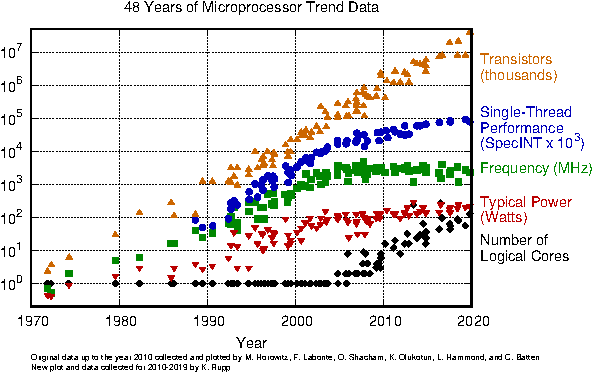
\includegraphics[width=\textwidth]{48-years-processor-trend.pdf}
    \caption{Trends in microprocessor development \cite{rupp2020trends}.} \label{fig:1}
\end{figure}

Beginning with the physical limitations, we can see that the clock speed has plateaued.
This is likely due to several factors: the capacitance of the transistors and the time needed to charge/discharge them and the limitations on transistor dielectric breakdown combined with chip design temperatures.
If we can keep the chips cooler, well below their design temperature we can increase the clock speed.
We will revisit the concept of chip thermal dissipation later.
What is interesting is that transistor density is continuing Moore's Law of exponential growth and will likely continue \cite{anthony2016transistors}.

Using the data from Rupp \cite{rupp2020trends}, we can estimate future performance in general computation (See Fig.~\ref{fig:2}).

\begin{figure}
    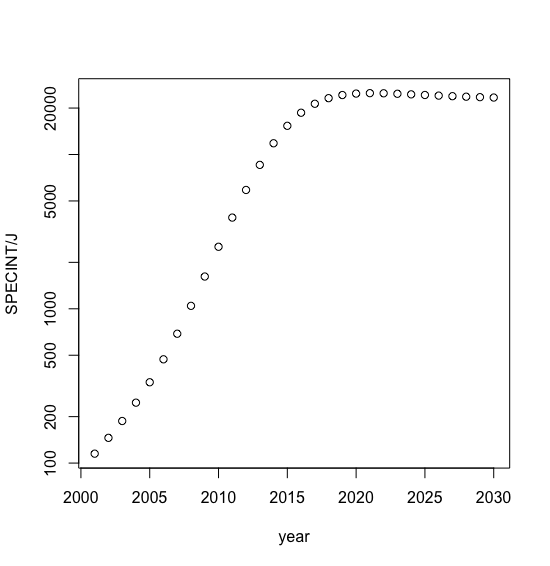
\includegraphics[width=\textwidth]{Processor Forecast.png}
    \caption{Fitted model of of computations per unit energy consumed. This is based upon \cite{rupp2020trends}.} \label{fig:2}
\end{figure}

%%%%%%%%%%%%%%%%%%%%%%%%%%%%%%%%%%%%%%%%%%%%%%%%%%%%%%%%%%%%%%%%%
% Trends in Mining Efficiency
%%%%%%%%%%%%%%%%%%%%%%%%%%%%%%%%%%%%%%%%%%%%%%%%%%%%%%%%%%%%%%%%%
\subsection{Trends in Mining Efficiency}

We can see similar fundamental limitations in mining performance as we can see in general computation.
Using the data collected by Kufoglu and Ozkuran \cite{kuf2019mining}, we can create a similar plot as to Figure~\ref{fig:2} (See Fig.~\ref{fig:3}).
Their original dataset was updated with a selection of more recent miners, Table~\ref{tbl:1}.

\begin{table}
    \caption{Selection of more recent bitcoin miners and their efficiency.}\label{tbl:1}
    \begin{tabular}{|l|l|l|l|}
        \hline
        Manufacturer &  Model   & Efficiency [J/TH] & Release Date   \\
        \hline
        AntMiner     & S15      &57                 & 11/11/2018     \\
        AntMiner     & S17      &39.5               & 19/04/2019     \\
        AntMiner     & S19      &34.5               & 01/05/2020     \\
        AntMiner     & S19j     &36.11              & 01/06/2021     \\
        AntMiner     & S19 Pro  &29.55              & 01/05/2020     \\
        AntMiner     & S19j Pro &30.5               & 01/06/2021     \\
        AntMiner     & S19 XP   &21.5               & 1/2/2022 (est) \\
        \hline
    \end{tabular}
\end{table}

\begin{figure}
    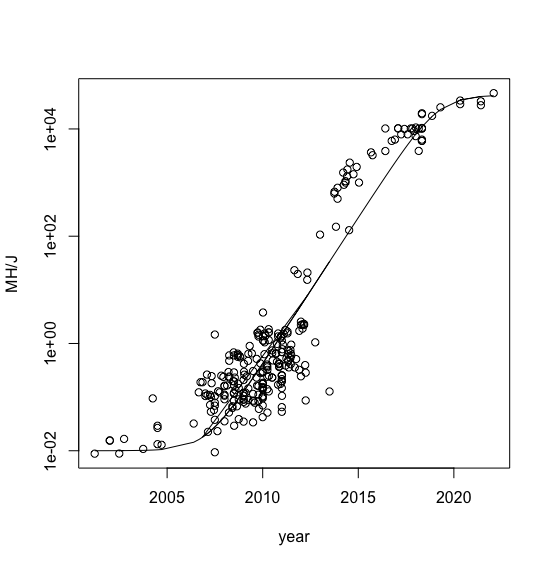
\includegraphics[width=\textwidth]{BTC Mining Performance.png}
    \caption{Fitted model of of computations per unit energy consumed. This is based upon \cite{rupp2020trends}.} \label{fig:3}
\end{figure}

The fitted curve in Figure \ref{fig:3} is given by,
\begin{equation}
    \eta(t) = A + \frac{K - A}{1 + e^{-B(t - M)}}
\end{equation}
Where the parameters are $A = 0.01 [MH/J]$, $K = 4.27\times 10^4 [MH/J]$,  $B = 1.26 [\frac{1}{a}]$, and $ M = 2019.2 [a]$.


%%%%%%%%%%%%%%%%%%%%%%%%%%%%%%%%
% Miner Tuning and Overclocking
%%%%%%%%%%%%%%%%%%%%%%%%%%%%%%%%
\subsubsection{Miner Tuning and Overclocking}
We can see with Figure~\ref{fig:3} that mining performance is clearly plateauing.
As a result of this there is an ever increasing trend for miner optimization.
For example Braiins OS for the older and programable Antminer S9 series, has implemented features such as chip specific autotunning to optimize hashrate efficiency for each chip individually \cite{braiins2021autotuning}.
Other open source miner firmware options exist, e.g. Hive OS, but they tend to be limited to older models due to firmware protection installed on newer miners by their manufacturers \cite{hiveos2020update}.

It seems that the miner manufactures are attempting to limit the performance of rigs that they sell to the public.
Bitmain for example builds a number of miners for themselves and could very easily write better firmware so that their miners are more productive than the ones they sell.
While this might be an effective short term strategy to maximize returns, in the long run and especially with miner performance plateauing, the manufacturers will face increased competition.

Furthermore, there is a tremendous lack of standardization with the different boards even with the same model from the same manufacturer.
These small dimensional fluctuations, make it very difficult to retrofit the miners with more efficient and dense cooling mechanisms.
The author developed a containerized liquid cooled system, but had to abandon the project because the miners kept on changing their dimensions.

%%%%%%%%%%%%%%%%%%%%%%%%%%%%%%%%
% Heat Removal
%%%%%%%%%%%%%%%%%%%%%%%%%%%%%%%%
\subsubsection{Heat Removal}
While the energy efficiency of bitcoin miners has plateaued, the increasing trend in smaller and smaller processors is going to impose a thermodynamic limit on the current designs.
Air as a heat transfer fluid is absolutely terrible.
It is characterized by a low density and a low Prandtl number, 0.7.
The Prandtl characterizes the preference of the fluid for thermal diffusivity $Pr < 1$ and momentum diffusivity $Pr \gg 1$.
Because liquids tend to be much more dense having a large momentum diffusivity greatly enhances heat transfer from the surface, with a much thinner thermal boundary layer.
This translates to needing much less surface area to remove an equivalent amount of heat.

In addition to the author's own work with immersion cooling, there has been a significant trend in the growth of this in bitcoin mining.
There are some drawbacks associated with using an oil dielectric for cooling.
\begin{itemize}
    \item Generally, they are flammable.
    \item They can have adverse reactions with board components shortening board life.
    \item They are expensive.
\end{itemize}

While recent immersion cooling operations have been relatively simple, they have done little optimization to increase performance.
For this next step, hash board standardization is absolutely critical.
What we will need is to separate the cooling liquid from the board circuitry.
This can readily be achieved using aluminum brazed plates sandwiched between the circuit board layers and using a coolant like either pure water or an ethylene glycol water mixture.
These are inexpensive and common coolants that are non combustible.
These coolants support a wide temperature operating range from $-45^{\circ}C$ -- $100^{\circ}C$.
If the objective is to limit chip temperature to $<90^{\circ}C$, then the coolant needs to be at most $<35-40^{\circ}C$ to support effective heat transfer at low enough temperatures to support safely overclocking the chips.

As chip transistor density continues to increase, air cooling will no longer be adequate to remove the heat generated during operation.
This will only exacerbate the drive toward more compact heat exchange surfaces with densities of plate side $>200\frac{m^2}{m^3}$.
Because of the tight dimensional tolerances needed in compact heat exchangers, boards will have to have consistent dimensions.

%%%%%%%%%%%%%%%%%%%%%%%%%%%%%%%%
% Power Usage Effectiveness
%%%%%%%%%%%%%%%%%%%%%%%%%%%%%%%%
\subsubsection{Power Usage Effectiveness}
The current method of air cooling has a very low Power Usage Effectiveness, PUE, $\approx 1.044$.
\footnote{This is based on private communication from Upstream Data, "2x 0.5 HP (0.745 kW) fans every 180 kW of PDU" (17 Nov 2021) and for an Antminer S19XP  which has 4 fans (assuming 2.7A @ 12V) ~ 130 W for 3.25 kW of 29.5 J/TH.}
PUE is the ratio of the total power of the system to the power sent to the miners.
Keep in mind this is using outside ambient air which is blown, filtered, through the miners.
If air cooled system is moved from cold climates, the miners have to be under clocked to keep the chip temperatures in specification.
If air conditioning is used then the PUE significantly increases.

The use of liquid cooling, including immersion, where the coolant is directly cooled in a cooling tower, reduces the PUE to $1.016$.
This is because the pumping of a liquid requires much less energy for an equivalent mass flow rate.
Even the use of the cooling tower fan to drive air for the ultimate heat sink is more efficient because the cooling tower is simply better engineered than the small computer fans on the miners.
If the miner coolant can be cooled directly with water, e.g. the ocean, the PUE is $1.01$.
This is the limit of how efficient a mining system can be.

The PUE is important in the economic analysis because it is the energy overhead on top of the energy used for mining.
While it is a small quantity in bitcoin mining applications, a 2.5--4\% improvement in a process's energy efficiency is non trivial.

%%%%%%%%%%%%%%%%%%%%%%%%%%%%%%%%%%%%%%%%%%%%%%%%%%%%%%%%%%%%%%%%%%%%%%%%%%%%%%%%%%%%%%%%%%%%%%%%%%%
% Bitcoin's Marginal Utility
%%%%%%%%%%%%%%%%%%%%%%%%%%%%%%%%%%%%%%%%%%%%%%%%%%%%%%%%%%%%%%%%%%%%%%%%%%%%%%%%%%%%%%%%%%%%%%%%%%%
\section{Bitcoin's Marginal Utility}
Now that we have covered some of the more granular details necessary for the foundations of the overall economic model, we have one more foundation to set.
That foundation is to establish a consistent and stable metric for which to evaluate the value of the bitcoin mined.
We will first look at estimating the marginal utility as being derived from on chain metrics.
Then we will look at establishing a more absolute measure.

%%%%%%%%%%%%%%%%%%%%%%%%%%%%%%%%%%%%%%%%%%%%%%%%%%%%%%%%%%%%%%%%%
% On Chain Metrics
%%%%%%%%%%%%%%%%%%%%%%%%%%%%%%%%%%%%%%%%%%%%%%%%%%%%%%%%%%%%%%%%%
\subsection{On Chain Metrics}
Before we delve too far into developing the on chain metrics for marginal utility, we need to look at the process of how a block is discovered.
I do not use the word mined, because it is not mined, and even in traditional mining accessing the mineral/ore underground is a process of discovery.
To be awarded a block a miner has to generate a random number called a nonce, number used once. and combine that into a specific structured 80 byte packet of data, the block header.
The header is then hashed generating a unique 32 byte (256 bit) number for that data.
The hashed number has to have a value less than target number, $target$.
If the hashed value is less than the target that miner is awarded the block reward, called the coinbase.

The target is computed by:
\begin{equation}
    Target=\frac{MaxTarget}{Difficulty}=\frac{2^{224}}{Difficulty}. \label{eq:1}
\end{equation}

The max target was set in the genesis block with a byte string of ``1d00ffff'' and the initial difficulty for the first 2015 blocks was 1.
\footnote{There is an off-by-one bug in the source code where the target is recomputed every 2015 blocks instead of 2016 blocks.}

After the first 2015 blocks were mined, the target number was adjusted in the first difficulty adjustment.
The difficulty is adjusted every 2015 blocks so that the next 2015 blocks will take an anticipated 14-days,
\begin{eqnarray}
    Difficulty_{new} &=& Difficulty_{prev}\frac{\Delta t_{nom}}{\Delta t_{prev}}, \label{eq:2} \\
    \Delta t_{nom}   &=& 2016 [blocks] \cdot 600[\frac{s}{block}]. \\
\end{eqnarray}
The new difficulty is $Difficulty_{new}$.
The previous blocks difficulty is $Difficulty_{prev}$.
The nominal times between blocks is $\Delta t_{nom}$.
And $\Delta t_{prev}$ is the difference in time between the first block and the last block of that difficulty period.

We can now define the probability of finding the next block $p_i$ as being,
\begin{definition} \label{def:1}
    The probability of finding a hash with a value less than the $Target$ is:
    \begin{equation}
        p_i = \frac{Target}{2_{256}}.
    \end{equation}
\end{definition}

We can express Definition \ref{def:1} in terms of $Difficulty$ through Equation \ref{eq:1} as,
\begin{equation}
    p_i = \frac{1}{2^{32}Difficulty_i}. \label{eq:3}
\end{equation}

%%%%%%%%%%%%%%%%%%%%%%%%%%%%%%%%
% Transmission Probability
%%%%%%%%%%%%%%%%%%%%%%%%%%%%%%%%
\subsubsection{Transmission Probability}
There are a number of similarities between radioactive $\beta^-$ and $\alpha$ decay and bitcoin mining.
From a quantum prospective the occurrence of decay occurs when the wave function has a small portion that exists outside of energy well of the nucleus.
These probabilities are incredibly small and are independent from similar processes in other nuclei.

This very is similar to how the hash for the next block reward is found.
We could think of a hash being generated as a wave function propagating from the CPU to the network.
This hash has a certain potential $p$ and must tunnel past an infinitely thin barrier of a potential $c_0 \delta(x)$.
We will use a wave equation of the form:
\begin{equation}
    -\frac{1}{2}\psi''(x) + c_0 \delta(x) \psi(x) = 0 \label{eq:4}
\end{equation}
Equation \ref{eq:4} has the following solution:
\begin{equation}
    \psi(x) =\left\{
    \begin{array}{ll}
        e^{i p x} + r e^{-i p x} & x < 0 \\
        t e^{i p x} & x > 0 \\
    \end{array}
    \right.
\end{equation}

The transmission probability, $T = t^*t$ is:
\begin{equation}
    T = \frac{1}{1+\frac{c_0^2}{p^2}}. \label{eq:5}
\end{equation}
Which if $c_0 \gg p$ equation \ref{eq:5} becomes:
\begin{equation}
    T = \frac{p^2}{c_0^2}. \label{eq:6}
\end{equation}
With equation \ref{eq:6}, we have recovered Definition \ref{def:1}, with the quantum potentials being, $p = \sqrt{Target}$ and $c_0 = 2^{128}$.

%%%%%%%%%%%%%%%%%%%%%%%%%%%%%%%%
% Block Discovery as a Poisson Process
%%%%%%%%%%%%%%%%%%%%%%%%%%%%%%%%
\subsubsection{Block Discovery as a Poisson Process}
Mathematically we characterize the process of radioactive decay as a Poisson Point Process as it satisfies the four conditions defining a Poisson process.
\begin{enumerate}
    \item Independent increments: the numbers of arrivals occurring in the disjoint intervals of time are independent.
    \item Stationary increments: the number of arrivals occurring in a given time interval depends only on the length of the interval.
    \item The probability of one arrival occurring in a time interval of length $\delta t$ is $H \delta t + o(\delta t)$ for $\delta t \rightarrow 0$.
    \item The probability of two or more arrivals occurring in a time interval of length $\delta t$ is $o(\delta t)$ for $\delta t \rightarrow 0$ \cite{tijms2003first}.
\end{enumerate}
\footnote{For processes with infinitesimally small transition rates, $1 - e^{-H} = h - \frac{h^2}{2!} + \frac{h^3}{3! + \ldots = h + o(h)}$ as $h \rightarrow 0$\cite{tijms2003first}.}
We note that the quantum state transitions occur at infinitesimally small probabilities with each isotope being independent of all of the other isotopes.

The for bitcoin we observe that the transmission probabilities are fixed by Definition \ref{def:1} or equivalently equation \ref{eq:3}.
The generation of a suitable has follows the exact same statistical process as radioactive decay and it similarly satisfies the four conditions of a Poisson process.

We note that the transmission probability of a winning block is defined by equation \ref{eq:3} and is uniform for all processors generating all hashes within a given difficulty epoch $Difficulty_i$.
Because the transmission probability is uniformly distributed expected time to discover a block for $k$ hashes is, 
\begin{equation}
    E(S_k - S_{k - 1}| N(t) = n) = \frac{t}{n + 1}.\mbox{\cite{tijms2003first}}
\end{equation}
Where $S_k$ is the random variable of the inverse hash rate for $1 < k < n$ attempts.

Given that the number of hashes to discover a bock, $n$, is defined as $n \equiv \frac{1}{p_i}$ and $t$ is the observed time between blocks.
Because the hash rate, $H$, is defined based upon the arrival of new blocks, we will assume that it is constant for a given block.
Thus it will be a piecewise continuous step function for each block in the blockchain.
We can describe the mean of this function as being,
\begin{equation}
    \frac{1}{t_N - t_0}\int_{t_0}^{t_N} dt H(t) =  \frac{1}{N}\sum_i^N H_i = \langle H \rangle. \label{eq:7}
\end{equation}
Where the first blocks beginning time is $t_0$ and the $N^{\mbox{th}}$ block's discovery (end) time is $t_N$.

From Theorem 1.3.1 of \cite{tijms2003first}, we can describe the stepwise non stationary Poisson process for $t,\Delta t >0$ as,
\begin{equation}
    P\lbrace N(t + \Delta t) - N(t)= n\rbrace = \frac{(\langle H \rangle \Delta t)^n}{n!}e^{-\langle H \rangle \Delta t}\label{eq:8}
\end{equation}
Where $N$ is the random variable of the number of hashes and $\Delta t$ is some positive time step.

By Theorem 1.1.1 of \cite{tijms2003first}, the expected number of hashes is,
\begin{eqnarray}
    \langle N \rangle &=& \langle H \rangle \Delta t \\
    \langle N \rangle &=& 2^{32} \Delta t \sum_i \frac{Difficulty_i}{\Delta t_i} \\
\end{eqnarray}
Where $\Delta t = \sum_i \Delta t_i$.

%%%%%%%%%%%%%%%%%%%%%%%%%%%%%%%%
% Measuring Time
%%%%%%%%%%%%%%%%%%%%%%%%%%%%%%%%
\subsubsection{Measuring Time}
Bitcoin presents us with an interesting consequence of how the blocks are created, there is a time stamp for each block.
This timestamp can have a significant amount of error in it, approximately an hour behind to two hours ahead of network consensus time.
So it is entirely possible and, in fact, not uncommon to have a negative time difference between timestamps.
This does not work with the derivation of the Poisson process for block discovery as time and time steps are defined only on the positive half-line.

Fortunately, Bitcoin has a hard stop defining the allowed zero time for each block, the Median Time Past, MTP, rule \cite{bitcoin2021core}.
This rule requires that the timestamp of a new block be greater than the median timestamp of the previous 11 blocks.
When we measure the time step for a block it is always with reference to this number.
We will assume that the median block height has the median timestamp.
This is not an entirely accurate assumption but considering the inaccuracies in measuring time it is acceptable.
\begin{definition} \label{def:2}
    We express the time step for a particular block as,
    \begin{equation}
        \Delta t_i = \frac{nTime_i - Mdn_{i,11}}{6}
    \end{equation}
    Where $\Delta t_i$ is the $i^{\mbox{th}}$ time step, $nTime_i$ is the $i^{\mbox{th}}$ block's timestamp, and $Mdn_{i,11}$ is the median of the previous 11 blocks to the $i^{\mbox{th}}$ block.
\end{definition}

We observe that by Definition \ref{def:2} it is impossible to have a negative time step because the MTP rule invalidates any blocks which would have a negative time step.
Additionally, when we look at the data contained in the blockchain, we find that $\Delta t_i \sim \mbox{Gamma}(\alpha, \beta)$ and that the hashrate is $H_i \sim \mbox{Inv-Gamma}(\alpha_H, \beta_H)$.

%%%%%%%%%%%%%%%%%%%%%%%%%%%%%%%%%%%%%%%%%%%%%%%%%%%%%%%%%%%%%%%%%
% Computing Marginal Utility
%%%%%%%%%%%%%%%%%%%%%%%%%%%%%%%%%%%%%%%%%%%%%%%%%%%%%%%%%%%%%%%%%
\subsection{Computing Marginal Utility}
To establish what the marginal utility is, we need to have a solid metric for measuring utility that is absolute in its measure and is a conserved quantity.
During our quantum mechanical discussion we showed that  hashes, through the conservation of their current, are conserved.
This is an absolute measure and we could use it to establish utility, however, this is only valid on chain.
We need a metric that is referenced to an absolute off chain.

In Proof-of-Work coins, the hashes represent the proof of work.
Because of the incredibly low transmission probability of a hash, there is a significant amount of computational effort that has to be expended to find the winning hash.
This computational effort requires two things: capital investment in the equipment and energy to power the equipment.
Energy is by far the single most important consideration in bitcoin mining.
We previously related energy to hashes using historical data of bitcoin miner performance.
So, we will adopt that function to estimate the utility of bitcoin in the real world.

We now have everything that we need to define the per block marginal utility of bitcoin,
\begin{definition}\label{def:3}
    We define the marginal utility of bitcoin referenced to the nominal block as,
    \begin{equation}
        \lambda_{\mbox{\bitcoin},i} \equiv \frac{H_i 600}{Coinbase_i \eta(t_i)}.\label{eq:9}
    \end{equation}
    Where for the $i^{\mbox{th}}$ block, $lambda_i$ is the marginal utility [MJ/BTC], $H_i$ is the hashrate [TH/s], 600 is the number of seconds between nominal blocks, $eta(t_i)$ is the miner efficiency [MH/J], and $Coinbase$ is the sum of the {\tt utxos} [satoshi] in the block's first transaction, {\tt nTxOut}=0.
    The term {\tt utxo} stands for unspent transaction output. The $Coinbase_i$ needs to be divided by $10^8$ to convert from satoshi to BTC.
\end{definition}


%%%%%%%%%%%%%%%%%%%%%%%%%%%%%%%%%%%%%%%%%%%%%%%%%%%%%%%%%%%%%%%%%%%%%%%%%%%%%%%%%%%%%%%%%%%%%%%%%%%
% Mining Economics
%%%%%%%%%%%%%%%%%%%%%%%%%%%%%%%%%%%%%%%%%%%%%%%%%%%%%%%%%%%%%%%%%%%%%%%%%%%%%%%%%%%%%%%%%%%%%%%%%%%
\section{Mining Economics}
To begin an economic analysis we need to first define what it is that we are modeling.
A bitcoin mining operation will have to convert bitcoin into fiat currency in order to be able to repay loans, pay for electricity, and pay employees.
An alternative to converting accumulated bitcoin to fiat is to use the mined bitcoin as collateral for a loan to pay for operations.
For the sake of simplicity we will look at a conventional mining operation that is funded through debt and equity with the fraction of equity being $\alpha$ and the fraction of debt being $1 - \alpha$.

%%%%%%%%%%%%%%%%%%%%%%%%%%%%%%%%%%%%%%%%%%%%%%%%%%%%%%%%%%%%%%%%%
% Cost of Energy
%%%%%%%%%%%%%%%%%%%%%%%%%%%%%%%%%%%%%%%%%%%%%%%%%%%%%%%%%%%%%%%%%
\subsection{Cost of Energy}
Energy is the single largest cost for bitcoin mining operations.
It's cost is also not a constant value and can be relatively inelastic.
The use of power in grid connected applications can be a significant friction point for miners and their host countries.
In off grid applications such as flare gas operations, the flaring of excess natural gas from oil wells imposes a non trivial cost on the oil rig operators.
Each of these two scenarios have very different considerations in how the miners are operated and how capital is recovered and costs realized.

%%%%%%%%%%%%%%%%%%%%%%%%%%%%%%%%
% Grid Integration
%%%%%%%%%%%%%%%%%%%%%%%%%%%%%%%%
\subsubsection{Grid Integration}
Grids, especially in well developed markets, are very complex and have even more complex markets.
However, this complexity does open up some options where there is no discovery mechanism for the price of power.
A Purchase Power Agreement (PPA) is typically negotiated with an agreed upon price of power and can contain an option for demand response.
Demand response is when a consumer voluntarily shuts down or restricts their operations in response to price signals \cite{iea2021demand}.

Because mining can have highly granular control over the clock frequency of the individual processors on the hash boards, a mining operation can have incredibly precise control over their power usage.
This control can be tied in real time to the economic value of mining bitcoin (using market price API data from an exchange), and with the realtime price of power.
For simplicity let us assume that the operator manages to negotiate a base power rate of $\$65/MW-hr$ \cite{eia2021elect}.
They then negotiate to begin demand response when the price of power reaches the realtime breakeven price using an agreed upon calculation.
For example using an S19XP, as of 13 Dec 2021, this would be around $\$470/MW-hr$, but floats based on the network difficulty and market price.

The miners would then regulate their hashrate to maintain that price.
They would first reduce their clock to the most efficient clock.
Then, they would continue throttling back to the minimum clock on the board.
For an initially overclocked miner, this could be on the order of 20-30\% power reduction and would be agreed upon in the PPA.
Meanwhile they would be paid for the power averted based on the power that they did not consume at the market price.

The next stage is to start shutting down miners after reaching certain price levels.
This option places thermal stresses on the chips and could shorten chip life.
Actually determining the lost economic use value is a very involved calculation.
This would require careful negotiation.

%%%%%%%%%%%%%%%%%%%%%%%%%%%%%%%%
% Power Plant Integration
%%%%%%%%%%%%%%%%%%%%%%%%%%%%%%%%
\subsubsection{Power Plant Integration}
In new power plant construction actually integrating the mining operation with the power plant can eliminate transmission losses and transmission costs.
In the United States transmission costs amount to approximately $\$11/MW-hr$ \cite{ier2021transmission}, while transmission losses are 6\% \cite{worldbank2021losses}.
This translates to an onsite cost of power of $\$50/MW-hr$.

In this situation the power plant is the primary source of power and the grid is the backup.
The mining operation would also benefit from directly accessing the power plant's water cooling system.
This would result in significantly less capital expenditure for the mining operations heat rejection system.
Depending on the ultimate heat sink and using liquid cooling, this could provide an additional 2.4--4\% savings in electricity use.

There is another synergy with collocating mining with a power plant.
If the mining operation is large enough compared to the power plant, it could prevent a plant trip on a loss of offsite power by providing the minimum required load to keep the plant running.
This would simplify grid restoration in large scale blackouts because the power plant would not have to be black started, it would already be running.

In areas where grid capacity is limited, such as the developing world, integrating mining with the power plant would enable the power plant to be sized larger (lower capital cost [$\$/kW$]).
In some cases having a minimum guaranteed power off take improves the ability to finance the project if there is not a sovereign PPA.
This minimizes the possibility of transmission interruption.

The author was present at a power plant in Central America where the main output breaker opened due to under voltage protection causing a plant trip.
The power plant (coal) had very specific actions that had to be executed rapidly to prevent steam pressure and tube wall temperature excursions.
The impact of these actions, only mitigate the damage to the boiler.
They do not prevent it.
They said that this happened at least once a week and would take them 12-24 hours to recover, if they didn't have significant tube damage.
Meanwhile, the already strained grid went down in the surrounding region because of the loss of 60 MW of generation from (2) units.

%%%%%%%%%%%%%%%%%%%%%%%%%%%%%%%%%%%%%%%%%%%%%%%%%%%%%%%%%%%%%%%%%
% Common Cost Basis
%%%%%%%%%%%%%%%%%%%%%%%%%%%%%%%%%%%%%%%%%%%%%%%%%%%%%%%%%%%%%%%%%
\subsection{Common Cost Basis}
This is a very complex problem to tackle.
We are dealing with local currency, local currency inflation, changes in network hashing power, using bitcoin as a currency, tax implications of purchases using bitcoin, taking loans against bitcoin to prevent taxable events, volatile exchange rates, etc.
The reason why we spent so much time formally developing the marginal utility of bitcoin in terms of $[MJ/\bitcoin]$ was to alleviate as much of the complexity as we could by providing a common measurable reference indicator.

While $[MJ]$ and $[kW-hr]$ are both units of energy, we need to keep these concepts separate in terms of how and where they fit into the model.
When referring to economic utility, the unit will always be $[MJ]$ it could also be written as $[MJ_U]$ to make the distinction more explicit.
Measurements of electrical energy will always follow the SI convention with base units of $[W-hr]$, appended with the appropriate prefix denoting the order of magnitude.

We will look at converting things priced in local currency units to an energy basis, instead of traditional deflators such as the Consumer Price Index, CPI.
Then we will develop a model for the net return on mining over the economic life of a miner.
We will develop a method to minimize the tax liability in jurisdictions where bitcoin is treated as a commodity instead of a currency.

%%%%%%%%%%%%%%%%%%%%%%%%%%%%%%%%
% Energy Price Index
%%%%%%%%%%%%%%%%%%%%%%%%%%%%%%%%
\subsubsection{Energy Price Index}
Energy is central to the level of economic activity in which we engage in.
From a first law of thermodynamics perspective, this is intuitive as \emph{ALL} action is constrained by the available energy.
The impact and roll of energy can be measured using traditional econometrics.
In fact, 80\% of all economic activity is derived from the useful work input into the economy \cite{ayers2009engine}.
And, the price of energy is the single most important factor affecting economic growth \cite{ayers2009engine}.

For these reasons and also for the derivation of bitcoins value in terms of energy it is not unreasonable to consider using the cost of all useful work $[\$/MJ]$ into an economy as the basis of the marginal utility of a currency.
In this case, exergy, useful work, is the unit of economic utility, just as it is for Bitcoin.
The problem that we have is that this econometric measure is not published anywhere and to develop it would take a considerable amount of effort.
Instead, we will use as a proxy the average price of electricity, as electricity is effectively pure exergy.
For the purposes of this paper we will use the average price of electricity for all sectors as the value of the dollar \cite{eia2021browser}.
To convert this into units of utility we will apply the following formula,
\begin{equation}
    \lambda_{\$}(t) = \frac{3.6[\frac{MJ_U}{kW-hr}]}{Price(t)[\$/kW-hr]}.\label{eq:10}
\end{equation}

In all analysis multiply any dollar priced item (including debt) by $\lambda_{\$}(t)$.
One will have to make a projection of $\lambda_{\$}(t)$, using a seasonally adjusted value.

%%%%%%%%%%%%%%%%%%%%%%%%%%%%%%%%
% Mining Revenue
%%%%%%%%%%%%%%%%%%%%%%%%%%%%%%%%
\subsubsection{Mining Revenue}
The projection of mining revenue especially when considering it in terms of fiat currency is a very difficult thing to model.
The average miner reward can be expressed as,
\begin{equation}
    \langle Reward_i \rangle = \frac{Difficulty_0}{Difficulty_i}\langle Reward_0 \rangle
\end{equation}

If we combine this with Definition \ref{def:3}, we can express the utility $\langle U_i \rangle$ generated in the $i^{\mbox{th}}$ period as being,
\begin{eqnarray}
    \langle U_i \rangle &\equiv& \lambda_{\bitcoin, i} \langle Reward_i \rangle \\
    \langle U_i \rangle &=& \frac{\eta(t_0) Coinbase_0}{\eta(t_i)Coinbase_i} \langle U_0 \rangle \\ \label{eq:11}
\end{eqnarray}
Where $\eta(t_i)$ is the miner efficiency and $Coinbase_i$ is the blocks coinbase defined in equation \ref{eq:9}.
It is interesting to note that the average utility produced by each block is only a function of the coinbase and the efficiency of the miner, relative to the current state of the art.
The coinbase is fairly predictable, although the miner fees are going to play an ever increasing fraction of the coinbase.
And, barring any drastic technological changes, miner performance has plateaued.

Equation \ref{eq:11} can be appropriately discounted over the lifetime of the facility to provide and equivalent utility today.
The selection of the discount rate is very important and should not be done using conventional values, especially if any bitcoin is used in making capital purchases.
The reason why is that bitcoin is a long time preference currency \cite{ammous2018bitcoin}.
If a facility is purchasing using bitcoin, the value of the purchase less its costs has to be greater than the bitcoin used to make the purchase.
Because if one is investing any capital the alternative is to buy and hodl bitcoin.
The investment has to beat that.
For this reason and because utility is a conserved quantity, we express the total utility, $U_{total}$, as being,
\begin{equation}
    U_{total} = \sum_i \langle U_{in,i} \rangle - U_{expenses,i}\label{eq:12}
\end{equation}
Where $U_{in,i}$ is the utility defined in equation \ref{eq:11} and $U_{expenses,i}$ is sum of all of the expenses incurred in that period of time.

%%%%%%%%%%%%%%%%%%%%%%%%%%%%%%%%
% Minimizing Tax Liability
%%%%%%%%%%%%%%%%%%%%%%%%%%%%%%%%
\subsubsection{Minimizing Tax Liability}
Because of the tax complications with different jurisdictions, we will focus on the United States as it is now the single largest home to bitcoin mining.
The Internal Revenue Service, IRS, taxes bitcoin as a capital investment through capital gains.
We will use a tax rate of 20\%, $\eta_{tax} = 20\%$.
The total quantity of bitcoin needed to make a purchase, $N_{total}$ is,
\begin{equation}
    N_{total} = \frac{N_{purchase}}{1-(1-\frac{CB}{price})\eta_{tax}}
\end{equation}
Where $CB$ is the cost basis, $price$ is the market price of bitcoin determined at the time of purchase, and $N_{purchase}$ is the number of bitcoin used to make the purchase.

If the cost basis of the bitcoin used is high enough, it makes sense to make the purchase directly with bitcoin.
If the bitcoin was acquired with a very low cost basis then 25\% more bitcoin will have to be sold to cover the 20\% capital gains.
We will assume the the latter case for further consideration as the former has trivial tax implications.

One would want to consider using Last In First Out Accounting, LIFO, accounting for the entity owning the miners.
Using a bitcoin collateralized loan would make sense, provided the total cost of the loan was less than the tax that was avoided in bitcoin terms.
For this strategy, the initial $U_{in,i}$ of equation \ref{eq:12} would be 0 as the revenue would go to repay the loan.
As of this writing, bitcoin collateralized loans are around 11\% APR for a renewable 1-year loan.

Where there is risk in this strategy is in the price movements of bitcoin.
If the price of bitcoin (in dollars) goes up, then the loan is repaid much much more quickly.
If the price of bitcoin goes down, then it will take longer for the loan to be repaid.
And, If the price goes down far enough, more bitcoin would be needed to provide adequate collateral.

%%%%%%%%%%%%%%%%%%%%%%%%%%%%%%%%%%%%%%%%%%%%%%%%%%%%%%%%%%%%%%%%%
% Accounting for Uncertainty
%%%%%%%%%%%%%%%%%%%%%%%%%%%%%%%%%%%%%%%%%%%%%%%%%%%%%%%%%%%%%%%%%
\subsection{Accounting for Uncertainty}
One of the failings of game theory and the concept of expected utility is that uncertainty is not formally taken into account with the model.
This was recently resolved by applying a statistical approach to game theory \cite{abel2021entropy}.
The result was that the uncertainty was accounted for with the economic Helmholtz potential \cite{abel2021entropy},
\begin{equation}
    F = U - T S. \label{eq:13}
\end{equation}
Where $F$ is the Helmholtz potential, $U$ is the utility, $T$ is the economic temperature, and $S$ is the entropy.
The total utility is one of any of the options, e.g. selecting the miner, site location, hodling bitcoin, selling bitcoin, leveraging bitcoin, fluctuations in the price of power, lack of availability of power etc.
All of the model's assumptions, priors, are represented as statistical distributions.
The model then samples the distributions and generates an estimate of the projects total utility, $U_{total}$.
The posterior distribution is the distribution of the $U_{total}$ from each sample.
The entropy is the uncertainty of the choice, measured using Shannon's information entropy of the economic model's posterior distribution.
The economic temperature, marginal utility of uncertainty can be taken directly as the value of capital expenditure for the project, $U_{expended}$.

This allows us to rewrite equation \ref{eq:13},
\begin{eqnarray}
    F &=& U_{total} - U_{expended} S, \\
    \frac{F}{U_{expended}} &=& \frac{\langle U_{total}\rangle}{U_{expended}} - S. \label{eq:14}\\
\end{eqnarray}
The selection criteria is to choose the option with the greatest Helmholtz potential per unit of utility expended.
It is important to note that the Utility Return on Investment, UROI, is $\frac{\langle U_{total}\rangle}{U_{expended}}$, and that it is modified to take into account uncertainty.
The temperature acts as a measure to discount the uncertainty of the project.
In this way a project with a high utility and high uncertainty, would be penalized much more than a project with a lower utility and a correspondingly lower uncertainty.

One caveat with this approach, the ability of being able to fully quantify the uncertainty is impossible as the entropy is not able to be measured \emph{ex ante}.
Only a best estimate can be made.

Equation \ref{eq:14} can just as easily be applied to the power plant economics.
The entropy needs to include the forced outage rate of dispatchable generation sources.
For non-dispatchable generators the power plant's output needs to be modeled with the probability distribution of the anticipated location's wind/solar characteristics.
The significantly larger entropy of wind/solar drastically penalizes their economic potential.
Reliability has a definite economic value.

%%%%%%%%%%%%%%%%%%%%%%%%%%%%%%%%%%%%%%%%%%%%%%%%%%%%%%%%%%%%%%%%%%%%%%%%%%%%%%%%%%%%%%%%%%%%%%%%%%%
% Conclusion
%%%%%%%%%%%%%%%%%%%%%%%%%%%%%%%%%%%%%%%%%%%%%%%%%%%%%%%%%%%%%%%%%%%%%%%%%%%%%%%%%%%%%%%%%%%%%%%%%%%
\section{Conclusion}

This paper has covered a significant breadth of topics ranging from quantum and statistical physics to Game Theory and statistical economics.
It is an effort to from first principles to derive the methodology of how to properly account for the economics of bitcoin mining.

There have been four major findings of this paper.
First, is the trends in processor performance and mining energy efficiency has plateaued due to reaching the physical limits of classical computing.
Second, is that the mining process of finding a hash with an integer value less than the target is fundamentally and mathematically equivalent to quantum tunneling as seen in radioactive decay.
Third, we found that this quantum state transition is governed as a Poisson Process and from this derived the marginal utility of bitcoin.
Finally, we created a method for how to formally and fully analyze the economic potentials of the different projects.

While the exposition of the different ideas was not necessarily easy, the conclusions proved to have simple and intuitive results.


%
% ---- Bibliography ----
%
\bibliographystyle{splncs04}
\bibliography{mining_economics.bib}

\end{document}
